\documentclass[dvipsnames]{article}
\usepackage{minted}
\documentclass[dvipsnames]{article}
\usepackage{amsmath,amsthm,amssymb}
\usepackage{graphicx}
\usepackage{hyperref}
\usepackage{textcomp}
% \usepackage{dsfont}
\usepackage{tabularx}
\usepackage{tikz}
\usepackage{physics}
\usepackage{changepage}% http://ctan.org/pkg/changepage
\usetikzlibrary{scopes,calc,arrows}
\usepackage{setspace}
\usepackage[makeroom]{cancel}
\usepackage{enumitem}
\usepackage[margin=1in]{geometry}
\usepackage[T1]{fontenc}
\usepackage[utf8]{inputenc}
\usepackage{tabularx,ragged2e,booktabs,caption}
\usepackage{wrapfig,lipsum,booktabs}
\usepackage{hanging}
\usepackage{multicol}
\usepackage{multirow}
\usepackage{blindtext}
\usepackage{booktabs}
\usepackage{color}
\usepackage{dcolumn}
% \usepackage{minted}
% \definecolor{light}{rgb}{0.35, 0.35, 0.35}
% \def\light#1{{\color{light}#1}}
\usepackage{mathtools}
\newcommand{\p}{\mathbb{P}}
\newcommand{\E}{\mathbb{E}}
\newcommand{\R}{\mathbb{R}}
\newcommand{\Var}{\operatorname{Var}}
\newcommand{\gr}{\textcolor{ForestGreen}}
\newcommand{\rd}{\textcolor{red}}


\title{IO Problem Set 2 (GPV)}
\author{Chris Ackerman\thanks{I worked on this problem set with Luna Shen, David Kerns, and Benedikt Graf}}
\date{\today}

\begin{document}
\maketitle
\begin{abstract}
  This problem set asked us to write code to implement the GPV algorithm on bid data from John's website. My write-up first outlines the approach I took, then has a brief discussion of data features/playing around with kernels, and finally plots the estimated density of private valuations against the observed bids. The appendix contains the full program that I ran.
\end{abstract}
\section{Overview}
For this problem set, I
\begin{enumerate}
\item Loaded the bid data from John's website.
\item Graphed the distribution of bids by each bidder to get a sense of what the data looked like.
\item Fit a nonparametric kernel to the aggregate bid data to see how it looked.
  \item Implemented the GPV algorithm on the data, by manually implementing a normal kernel density estimator of the distribution of bids and then inverting it to get estimated valuations.
\end{enumerate}
These function calls omit some helper functions for the GPV algorithm.
\begin{minted}{python}
    
if __name__ == '__main__':
    my_dir = "/home/chris/files/school/ucla/second_year/fall/io/pset2"
    os.chdir(my_dir)
    bid_data = load_bid_data(filename="PS3Data.csv")
    graph_bidder_data(bid_data=bid_data, filename='bidder_histogram.pdf', n_bins=50)
    graph_bids(bid_data=bid_data, filename='bid_density.pdf', bandwidth=0.5)
    density_support = np.linspace(2, 10, 500)
    estimated_density = estimate_values_density(
                                    B = bid_data[['Bidder 1', 'Bidder 2']].to_numpy()/2,
                                    kg = generate_uniform_kernel(),
                                    rhog = 1,
                                    kf = generate_uniform_kernel(),
                                    hg = 0.1,
                                    hf = 0.1,
                                    grid = density_support
    )
    graph_estimated_density(
                            density_support=density_support,
                            estimated_density=estimated_density,
                            filename='estimated_density.pdf'
    )
  \end{minted}
  \section{Bid Data}
  \begin{figure}[htp]
    \centering
    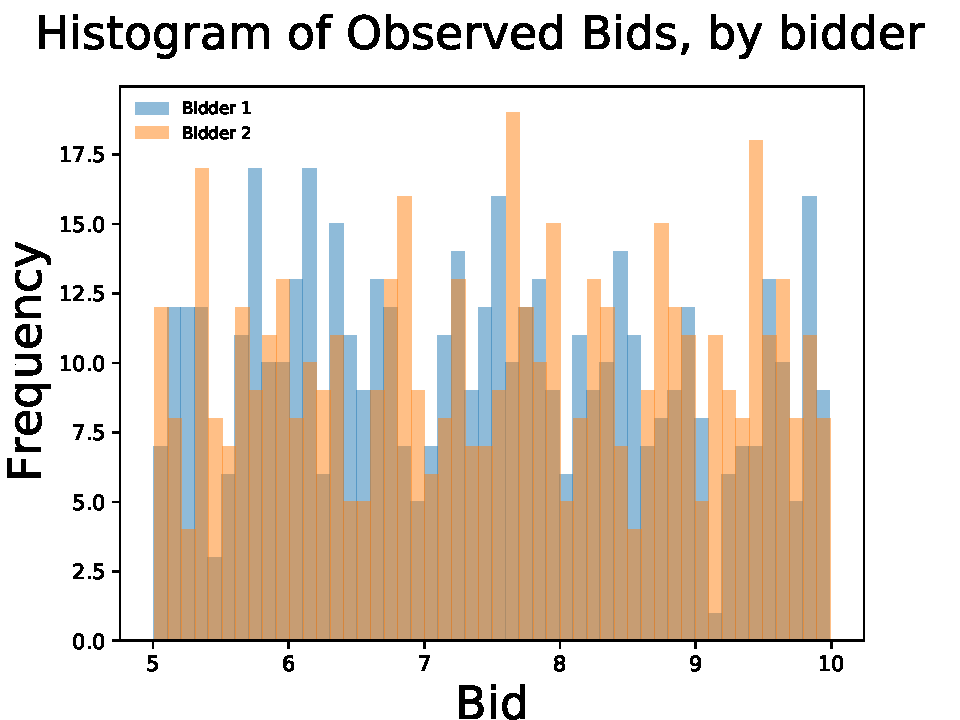
\includegraphics{bidder_histogram.pdf}
    \caption{This figure graphs a histogram of each bidder's bids. Each bidder has their own color, and the histograms look pretty much the same. Nothing too crazy here, but reassuring since we're assuming the bidders have independent private values drawn from the same distribution.}
  \end{figure}

  
  \begin{figure}[htp]
    \centering
    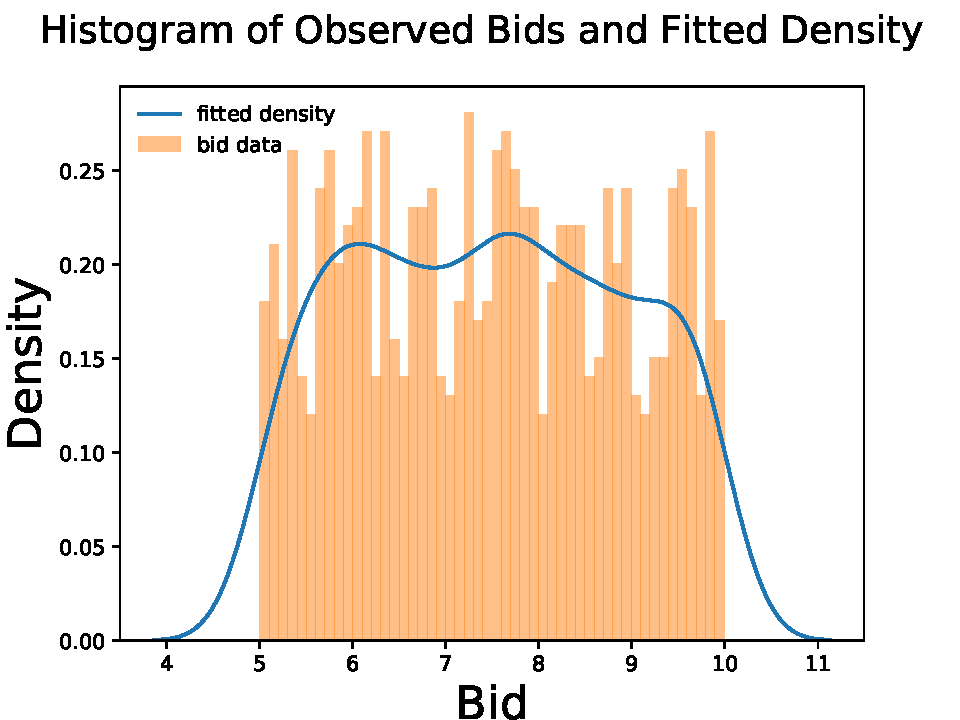
\includegraphics{bid_density.pdf}
    \caption{This figure pools the bid data from both bidders and fits a nonparametric density to the data. It is reassuring that the canned kernel density estimator that I'm using seems to do a reasonable job fitting the data.}
  \end{figure}

  \section{Estimated Valuations}
  \begin{figure}[htp]
    \centering
    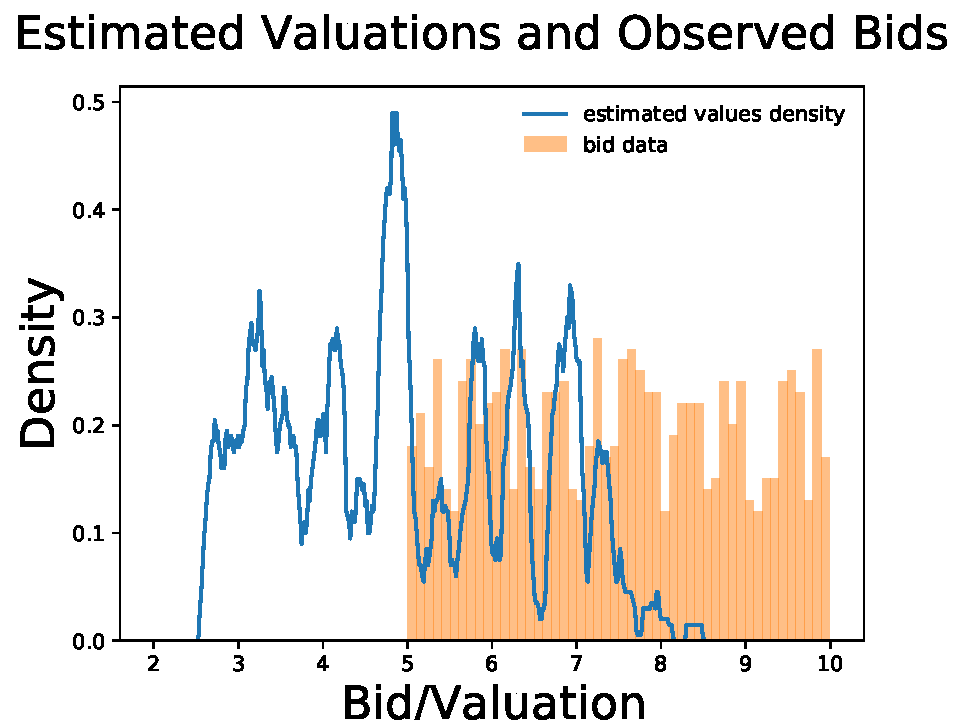
\includegraphics{estimated_density.pdf}
    \caption{This figure graphs the estimated valuations from the GPV algorithm against the observed bid data (included as a sanity check). It is concerning that the estimated density doesn't reach the top of the support of bids, since that indicates that bidders are sometimes bidding more than their valuation (which should never happen in equilibrium with a first price auction). However, the GPV paper does mention that their algorithm is biased near the edges of the distribution, so that is a possible explanation for the lack of estimated valuations above $\sim 8.5$.}
  \end{figure}
  \newpage
\inputminted{python}{GPV_code.py}
\end{document}
%%% Local Variables:
%%% mode: latex
%%% TeX-master: t
%%% End:
